\section{Lezione 15}%
\label{sub:Lezione 15}
\subsection{Dinamica nello spazio delle fasi.}%
\label{sub:Dinamica nello spazio delle fasi.}
Tipicamente si parte da un set di variabili differenziali della seguente struttura:
\[
    \vect{\dot{x}} = f(\vect{x}) 
.\] 
In cui $\vect{x}$  sono delle coordinate generalizzate, mentre le $f(\vect{x})$  sono delle funzioni di queste variabili tipicamente non lineari.
\begin{exmp}[Oscillatore armonico]
    \[\begin{aligned}
	& \dot{x}=v\\
	& \dot{v} = -\omega_0^2x
    .\end{aligned}\]
    In questo caso si prendono come coordinate $x$  e $v$  e si possono vedere le traiettorie nello spazio delle fasi.\\
    Prendendo ad esempio $\omega_0^2 = 1$  si scopre l'identità:
    \[
	\frac{\text{d} }{\text{d} t} (v^2+x^2) = 0
    .\] 
    Di conseguenza le traiettorie nello spazio delle fasi sono dei semplici cerchi.
    \begin{figure}[H]
    \centering
    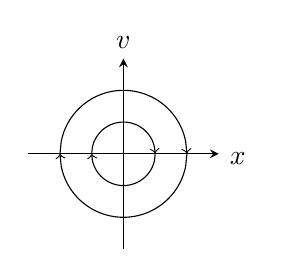
\begin{tikzpicture}
	\begin{axis}[
	    width=4cm,
	    height=4cm,
	    xmin= -3, xmax= 3,
	    ymin= -3, ymax = 3,
	    axis lines = middle,
	    x label style={at={(axis description cs:1.1,0.56)},anchor=north},
	    y label style={at={(axis description cs:0.5,1)},anchor=south},
	    xlabel={$x$},
	    ylabel={$v$},
	    xtick={0},
	    ytick={0},
	    xticklabel={},
	    yticklabel={},
	    ]

	    \addplot [domain=-2:2, samples=100, ->] {sqrt(4-x^2)};
	    \addplot [domain=-2:2, samples=100, <-] {-sqrt(4-x^2)};

	    \addplot [domain=-1:1, samples=100, ->] {sqrt(1-x^2)};
	    \addplot [domain=-1:1, samples=100, <-] {-sqrt(1-x^2)};

	\end{axis}
    \end{tikzpicture}
    \caption{\scriptsize Moto nello spazio delle fasi per un oscillatore armonico.}
    \label{fig:osc_armonico}
\end{figure}

\end{exmp}
\noindent
\begin{exmp}[Pendolo]
    \[\begin{aligned}
	& \dot{x}=v\\
	& \dot{v}=-\frac{g}{l}\sin (x) 
    .\end{aligned}\]
    Dobbiamo prima cercare le traiettorie per il quale si annullano $\dot{x}$ oppure $\dot{v}$ (le nurk lines). 
    \begin{itemize}
        \item $\dot{x}$ si annulla quando $v = 0$, quindi per tale retta si ha una nurk line.
	\item $\dot{v}$ si annulla con $\sin (x) = 0$, quindi avremmo delle nurk line verticali per i seguenti valori di $x$: 
	    \[
		x = k\pi  \qquad k \in \mathbb{Z}
	    .\] 
    \end{itemize}
    Anche in questo caso è noto che vi è un integrale del moto (la cui derivata rispetto al tempo è nulla): 
    \[
	E = \frac{1}{2}v^2 - \frac{g}{l}\left(\cos (x) + 1\right)
    .\] 
    Quindi possiamo disegnare delle linee di flusso nello spazio delle fasi semplicemente plottando al variare di $E$  la seguente:
    \[
	v = \pm \sqrt{2 \left( E + \frac{g}{l}(1 + \cos (x)) \right) } 
    .\] 
    \documentclass[crop,tikz]{standalone}% 'crop' is the default for v1.0, before it was 'preview'
\usepackage{pgfplots}
\usetikzlibrary{math}
\begin{document}
    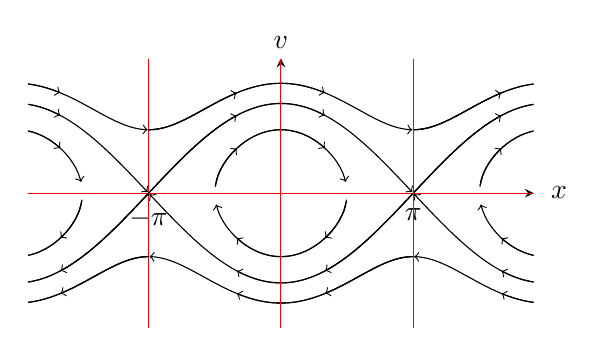
\begin{tikzpicture}
  	\tikzmath{\xa = 6; \y = 3;}
	\begin{axis}[
	    width=8cm,
	    height=5cm,
	    xmin= -\xa, xmax= \xa,
	    ymin= -\y, ymax = \y,
	    axis lines = middle,
	    x label style={at={(axis description cs:1.05,0.56)},anchor=north},
	    y label style={at={(axis description cs:0.5,1)},anchor=south},
	    xlabel={$x$},
	    ylabel={$v$},
	    xtick={0, pi, -pi},
	    xticklabels={$0$, $\pi$, $-\pi$},
	    ytick={0},
	    yticklabel={},
	    ]
	    %%%%%%%%%%%%%%%%%%%%%%%%%%%%%%%%%%%
	    %  Linea orizzontale (nurk line)  %
	    %%%%%%%%%%%%%%%%%%%%%%%%%%%%%%%%%%%
	    \addplot [domain=-\xa:\xa, samples=5, red] {0};
	    
	    \foreach \n in {-2*pi,0,2*pi} { % Vario "l'occhio" da visualizzare
		\foreach \s in {0.01,1,2} { % Traccio più linee per avere più punte di freccia
		    \foreach \E in {-1, 0 , 1} { % Vario l'energia per vedere le tre aree dello spazio delle fasi
			%%%%%%%%%%%%%%%%%%%%%%%%%%%%%%%%%%%%%%%%%%%%%
			%  Linee del moto al variare della energia  %
			%%%%%%%%%%%%%%%%%%%%%%%%%%%%%%%%%%%%%%%%%%%%%
		    	\addplot [domain= ( -pi-\n): ( pi-\n ) - 2*pi*\s/3, samples=100, ->] {sqrt( 2*(\E + 1 + cos(deg(x)) ))};
		    	\addplot [domain= ( -pi-\n) + 2*pi*\s/3: ( pi-\n ) , samples=100, <-] {-sqrt( 2*(\E + 1 + cos(deg(x)) ))};
		    }
		}
		%%%%%%%%%%%%%%%%%%%%%%%%%%%%%%%%%%
		%  Linee verticali (nurk lines)  %
		%%%%%%%%%%%%%%%%%%%%%%%%%%%%%%%%%%
	    	\addplot [red] coordinates {(\n/2, -\y) (\n/2, \y)};
	    }
	\end{axis}
    \end{tikzpicture}
\end{document}

    Notiamo in figura \ref{fig:15_pendolo} che nei punti 
    \[
        x = 2k\pi, \quad v = 0
    .\] 
    le linee di flusso si incrociano ma la dinamica del pendolo sembra presentare uno "spigolo": come se il moto rimbalzasse sull'asse $x$. Approfondiremo nel corso della lezione la natura di questi punti sella.
\end{exmp}
\noindent
In generale vale che:
\begin{redbox}{Linee di flusso nello spazio delle fasi}
    Dato un potenziale $U(x)$ possiamo disegnare delle linee di flusso ad energia fissata nello spazio delle fasi $v,x$ come:
    \[
	v = \pm \sqrt{2(E-U(x))} 
    .\] 
\end{redbox}
\noindent
\begin{exmp}[Moto in doppia buca]
Prendiamo un potenziale formato da una doppia buca asimmetrica, il moto nello spazio delle fasi è il seguente:    
\begin{figure}[H]
    \centering
    \begin{tikzpicture}
  	\tikzmath{\xa = 2; \y = 3; \lim = 1.6;}
	\begin{axis}[
	    width=7cm,
	    height=4cm,
	    xmin= -\xa, xmax= \xa,
	    ymin= 0, ymax = \y,
	    axis lines = middle,
	    x label style={at={(axis description cs:1.05,0.06)},anchor=north},
	    y label style={at={(axis description cs:0.5,1)},anchor=south},
	    xlabel={$x$},
	    ylabel={$U(x)$ },
	    xtick={0},
	    xticklabels={$0$},
	    ytick={0},
	    yticklabel={$0$},
	    ]
	    \addplot[domain=-3:3, samples=500]{((x+1)^2+0.3)*(x-1)^2};
	\end{axis}
    \end{tikzpicture}
    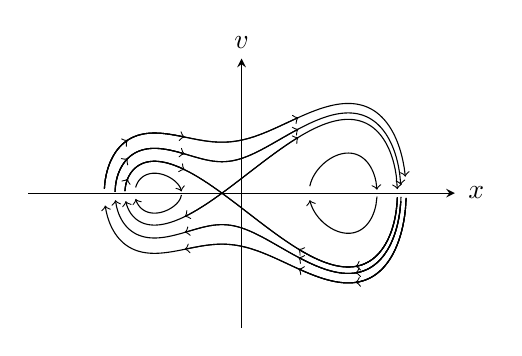
\begin{tikzpicture}
  	\tikzmath{\xa = 2; \y = 3; \lim = 1.6;}
	\begin{axis}[
	    width=7cm,
	    height=5cm,
	    xmin= -\xa, xmax= \xa,
	    ymin= -\y, ymax = \y,
	    axis lines = middle,
	    x label style={at={(axis description cs:1.05,0.56)},anchor=north},
	    y label style={at={(axis description cs:0.5,1)},anchor=south},
	    xlabel={$x$},
	    ylabel={$v$},
	    xtick={0},
	    xticklabels={$0$},
	    ytick={0},
	    yticklabel={},
	    ]
	    \foreach \s in {0,1,2, 2.5} { % Traccio più linee per avere più punte di freccia
		\foreach \E in {1.354 , 1.6, 2} { % Vario l'energia per vedere le tre aree dello spazio delle fasi
		    %%%%%%%%%%%%%%%%%%%%%%%%%%%%%%%%%%%%%%%%%%%%%
		    %  Linee del moto al variare della energia  %
		    %%%%%%%%%%%%%%%%%%%%%%%%%%%%%%%%%%%%%%%%%%%%%
		    %((x+1)^2+0.5)*(x-1)^2
		    %(-x^2/2*(1-x^2/2) + 0.3)
		    \addplot [domain= ( -\lim): ( \lim) - 2*\lim*\s/3, samples=300, ->] {sqrt( 2*(\E - ((x+1)^2+0.3)*(x-1)^2)  )};
		    \addplot [domain= ( -\lim) + 2*\lim*\s/3: ( \lim) , samples=300, <-] {-sqrt( 2*(\E - ((x+1)^2+0.3)*(x-1)^2) )};
		}
	    }
	    \addplot [domain= ( 0): ( 1.9), samples=200, ->] {sqrt( 2*(0.4 - ((x+1)^2+0.3)*(x-1)^2)  )};
	    \addplot [domain= ( 0): ( 1.9) , samples=200, <-] {-sqrt( 2*(0.4 - ((x+1)^2+0.3)*(x-1)^2) )};
	    \addplot [domain= ( -1.9): ( 0), samples=200, ->] {sqrt( 2*(1.2 - ((x+1)^2+0.3)*(x-1)^2)  )};
	    \addplot [domain= ( -1.9): ( 0) , samples=200, <-] {-sqrt( 2*(1.2 - ((x+1)^2+0.3)*(x-1)^2) )};
	\end{axis}
    \end{tikzpicture}
    \caption{\scriptsize Potenziale a doppia buca e linee di flusso per il moto nello spazio delle fasi. Notiamo la presenza di un punto sella che equivale ad un moto nel quale l'oggetto raggiunge il punto di massimo tra le buche con velocità nulla (in un tempo infinito). }
    \label{fig:15_double}
\end{figure}

Notiamo in figura \ref{15_double} che il moto può rimanere confinato all'interno di una delle due buche, esistono anche traiettorie che riescono ad entrare in tutte e due le buche "girando in tondo" nello spazio delle fasi. 
\end{exmp}
\noindent
In generale potremmo cercare un metodo per capire quali traiettorie scappano dal potenziale e quali invece rimangono confinate.
\subsection{Tecnica della stabilità lineare}%
\label{sub:Tecnica della stabilità lineare}
Prendiamo delle equazioni del moto del seguente tipo:
\[
    \begin{cases}
	\dot{x} = f(x, y) \\
	\dot{y} = g(x,y) 
    \end{cases}
.\] 
e supponiamo di aver identificato un punto $P_0=(x_0, y_0)$ tale per cui $\dot{x}=\dot{y}=0$.\\
La tecnica della stabilità lineare si basa sulla espansione delle equazioni del moto attorno al punto di equilibrio $P_0$.
\[\begin{aligned}
    & x = x_0 + \delta x\\
    & y = y_0 + \delta y
.\end{aligned}\]
Derivando queste due equazioni si ottiene: 
\[
    \begin{pmatrix} \delta\dot{x} \\ \delta\dot{y} \end{pmatrix} =
    \begin{pmatrix} 
	\partial_{x}f & \partial_{y}f\\
	\partial_{x}g & \partial_{y}g
    \end{pmatrix} 
    \begin{pmatrix} \delta x \\ \delta y \end{pmatrix} 
    \equiv 
    M 
    \begin{pmatrix} \delta x \\ \delta y \end{pmatrix} 
.\] 
A questo punto diagonalizzando la matrice $M$ si ottiene l'andamento del moto nello spazio delle fasi in un intorno del punto di stabilità $P_0$.
\[
    \text{det}\left|M-\lambda\mathbb{I}\right|=0
.\] 
Infatti ottenuto il set di $\lambda_i$ possiamo scrivere:
\[
    \delta \vect{x} = C_1\vect{D}_1e^{\lambda_1t} + C_2\vect{D}_2e^{\lambda_2t}
.\] 
Con $\vect{D}_i$ autovettori. Nel sistema di questi si ha che:
\[
    \dot{\vect{D}}  = \lambda  \vect{D}
.\] 
\subsection{Classificazione dei punti fissi}%
\label{sub:Classificazione dei punti fissi}
A seconda del segno degli autovalori possiamo riscontrare diverse situazioni:
\paragraph{Nodo stabile}%
\label{par:Nodo stabile}
Se gli autovalori sono entrambi negativi:
\[
    \lambda_1<\lambda_2<0
\] 
allora l'oggetto del moto cade nel punto $P_0$ esponenzialmente nel tempo (nello spazio degli autovettori $D_i$) come possiamo vedere in figura \ref{fig:figures-15_lambda-png}(a).
\paragraph{Nodo instabile}%
\label{par:Nodo instabile}
\[
    \lambda_1 > \lambda_2 > 0
.\] 
In questa situazione l'oggetto del moto si allontana esponenzialmente dal punto fisso (figura \ref{fig:figures-15_lambda-png}(b)).
\paragraph{Punto iperbolico}%
\label{par:Punto iperbolico}
\[
    \lambda_1<0<\lambda_2
.\] 
Questa è la situazione di punto sella accennata nelle sezioni precedenti (figura \ref{fig:figures-15_lambda-png}(c)).
\paragraph{Spirale stabile/instabile}%
\label{par:Spirale stabile}
\[\begin{aligned}
    & \lambda_1 = -\alpha+i\beta\\
    & \lambda_2=-\alpha-i\beta
.\end{aligned}\]
In questo caso l'oggetto spiraleggia fino a cadere nel punto, in questi casi tale punto è spesso chiamato attrattore (figura \ref{fig:figures-15_lambda-png}(d)).\\
Nel caso della spirale instabile cambia soltanto il segno di $\alpha$:
\[\begin{aligned}
    & \lambda_1 = \alpha+i\beta\\
    & \lambda_2= \alpha-i\beta
.\end{aligned}\]
Gli oggetti si allontanano spiraleggiando dal punto in questione (figura \ref{fig:figures-15_lambda-png}(e))
\paragraph{Punto ellittico}%
\label{par:Punto ellittico}
\[\begin{aligned}
    & \lambda_1 = i\beta_1\\
    & \lambda_2= -i\beta_2
.\end{aligned}\]
In questo caso gli oggetti ruotano attorno al punto fisso, se $\beta_1=\beta_2$ allora la traiettoria nello spazio delle fasi è una circonferenza (figura \ref{fig:figures-15_lambda-png}(f)).
\begin{figure}[H]
    \centering
    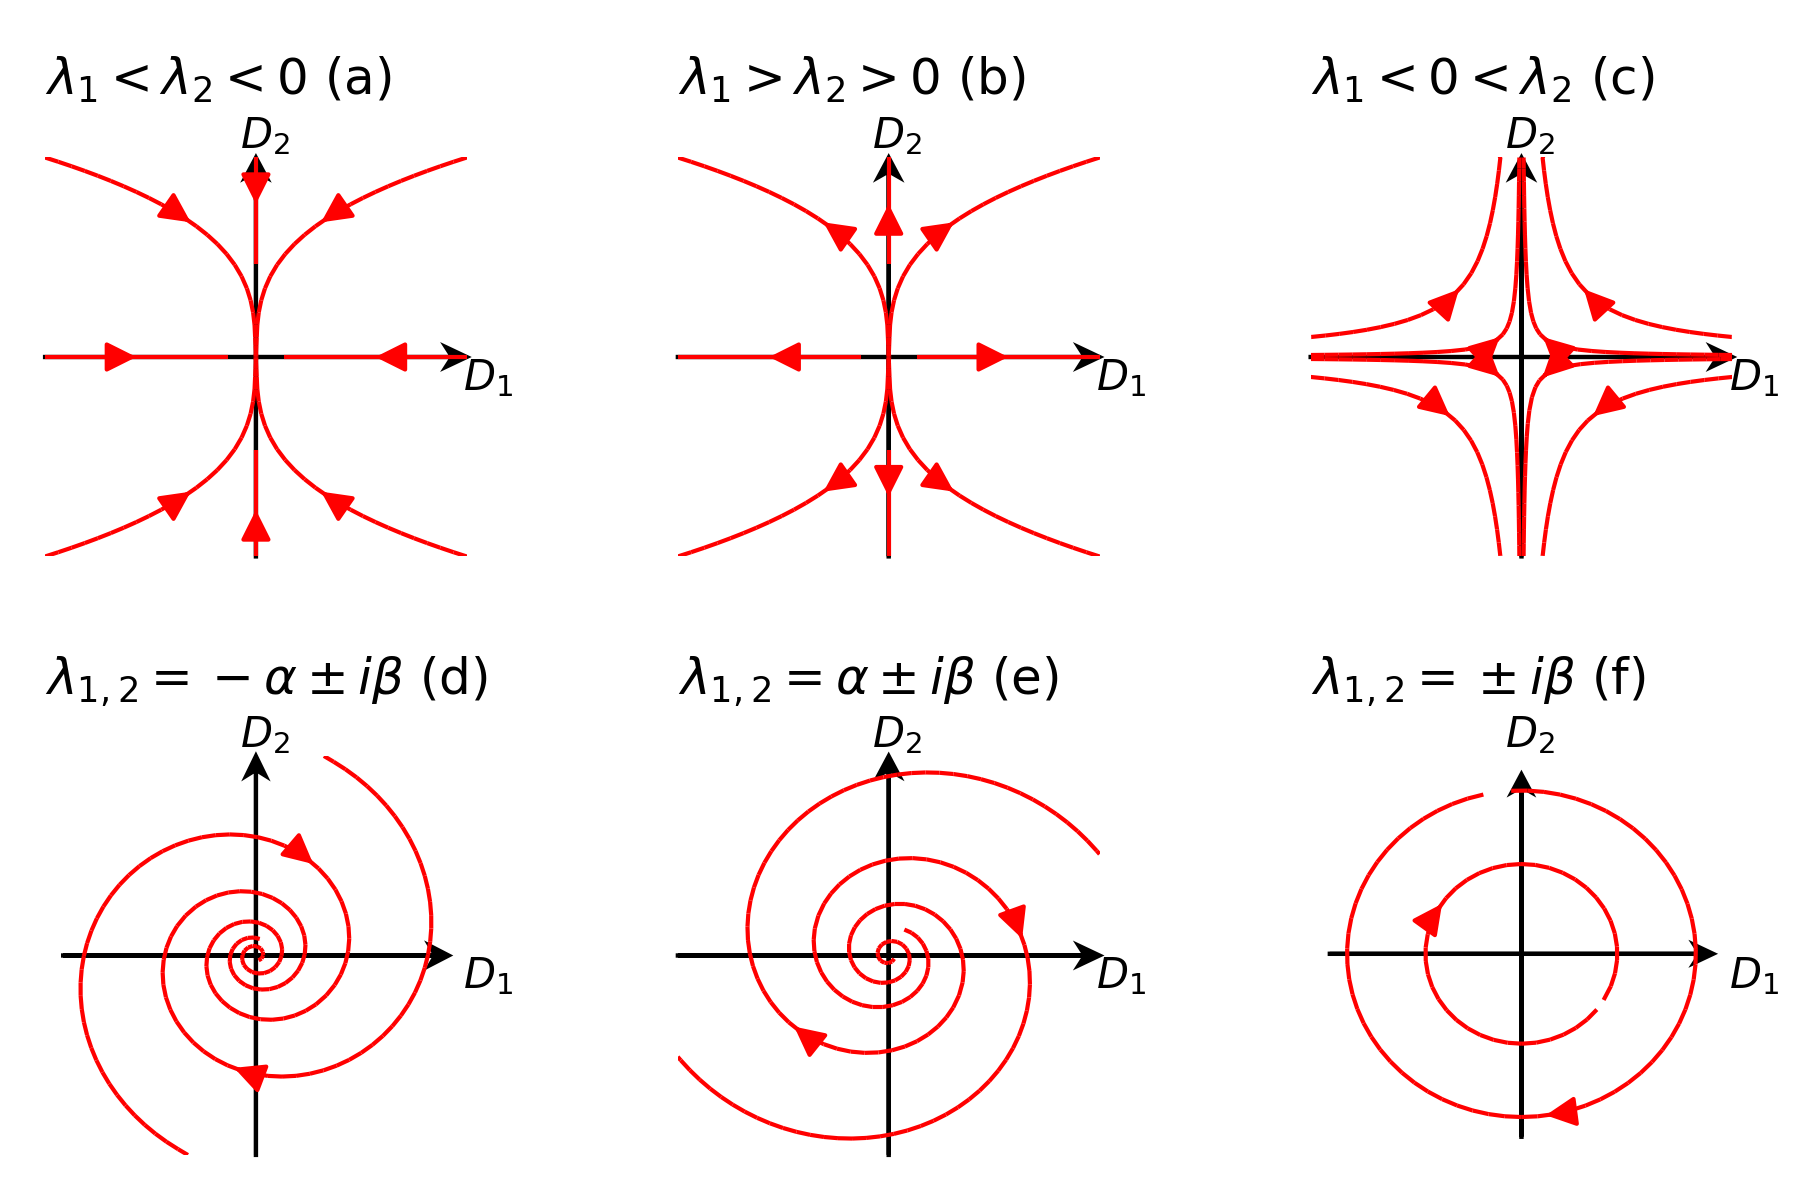
\includegraphics[width=0.5\textwidth]{figures/15_lambda.png}
    \caption{\scriptsize Tipi particolari di punti stabili nello spazio delle fasi.}
    \label{fig:figures-15_lambda-png}
\end{figure}
Un ultimo caso è dato dall'annullarsi di uno dei due autovalori, in tal caso il moto avviene lungo una retta nello spazio delle fasi.
\begin{exmp}[Osillatore smorzato]
    Prendiamo l'equazione del moto:
    \[
        \ddot{x}=-\omega_0^2x -\gamma\dot{x}
    .\] 
    Possiamo riscriverla nel seguente modo:
    \[
        \begin{cases}
 	    \dot{x} = v\\
	    \dot{v}=-\gamma v - \omega_0^2x           
        \end{cases}
    \] 
    L'unico punto di equilibrio per il sistema è $P_0 = (x_0 = 0, v_0 = 0)$.\\
    Possiamo cercare le Nurk line: 
    \[\begin{aligned}
	& \dot{x}=0 \implies  v = 0\\
	& \dot{v}=0 \implies  v = -\frac{\omega_0^2}{\gamma}x
    .\end{aligned}\]
    Abbiamo ottenuto due rette che dividono il piano in 4 parti. Sulla base di queste suddivisioni si potrebbe già indovinare come saranno le linee di flusso nello spazio delle fasi, è necessario infatti considerare che le Nurk lines corrispondono ad una variazione di segno di $\dot{x}, \dot{v}$, quindi ci indicano la direzione dell'oggetto nello spazio delle fasi.\\
    Graficando le linee e osservando la direzione degli oggetti nel piano potremmo già concludere che i corpi spiraleggiano attorno all'origine. Proviamo a vederlo con il metodo descritto in questa sezione.
    \[
	\begin{pmatrix} \delta\dot{x} \\ \delta\dot{v} \end{pmatrix} =
	\begin{pmatrix} 
	    0 & 1\\
	    -\omega_0^2 & - \gamma
	\end{pmatrix} 
	\begin{pmatrix} \delta x \\ \delta y \end{pmatrix} 
    .\] 
    \[
        \lambda  = \frac{-\gamma  \pm \sqrt{\gamma^2 - 4\omega_0^2}}{2}
    .\] 
    Quindi possiamo distinguere due situazioni:
    \begin{itemize}
        \item  $\gamma^2 - 4\omega_0^2 > 0$. \\
	In questo caso gli autovalori $\lambda_1, \lambda_2$ sono entrambi reali, quindi l'origine è un nodo stabile.
    \item $\gamma^2 - 4\omega_0^2 < 0$.\\
	In tal caso si ha che:
	\[
	    \lambda_{1,2} = -\frac{\gamma}{2} \pm i \omega
	.\] 
	Quindi in tal caso l'origine è un punto di spirale stabile.
    \end{itemize}
    Notiamo che in questo caso particolare, poiché la matrice delle derivate miste perde la dipendenza da $v$ e $x$, lo sviluppo lineare vale in tutto il piano e non soltanto in un intorno dell'origine.
\end{exmp}
\noindent
\begin{exmp}[Pendolo smorzato]
    L'equazione per il pendolo smorzato è:
    \[
        \begin{cases}
            \dot{x} = v\\
	    \dot{v} = - g /l\sin (x) - \gamma v
        \end{cases}
    \] 
    I nodi stabili sono tutti i punti tali che:
    \[\begin{aligned}
	& v_0 = 0\\
	& x_0 = n \pi
    .\end{aligned}\]
    Prendendo la matrice delle derivate miste si ha:
    \[\begin{aligned}
	\begin{pmatrix} \delta\dot{x} \\ \delta  \dot{v} \end{pmatrix} =&
	\left.	\begin{pmatrix} 
	    0 & 1 \\
	    -g /l \cos (x) & - \gamma
	\end{pmatrix} \right|_{x_0,y_0}
	\begin{pmatrix} \delta x \\ \delta v \end{pmatrix} \\
	=&
	\begin{pmatrix} 
	    0 & 1 \\
	    \pm g /l& - \gamma
	\end{pmatrix}
	\begin{pmatrix} \delta x \\ \delta v \end{pmatrix} 
    .\end{aligned}\]
    Dobbiamo distinguere tra il caso in cui nella matrice vi è il segno positivo da quello in cui nella matrice vi è il segno negativo, per entrambi i vasi si studia il sistema e si ottengono i seguenti risultati:
    \begin{itemize}
	\item Segno $+$ ($x_0 = (2n+1)\pi$):\\
	    $\lambda_1 < 0,  \lambda_2 > 0 \implies$ Punto sella.
	\item Segno $-$ ($x = 2n\pi$): 
	    \begin{itemize}
		\item $\gamma^2 / 4 > g /(4l)$: \\
		    $\lambda_1,\lambda_2 < 0 \implies$ Nodo stabile.
		\item $\gamma^2 / 4 < g /(4l)$: \\
		    $\lambda_{1,2} $ C.C. $\implies$ Spirale stabile.
	    \end{itemize}
    \end{itemize}
    \begin{figure}[H]
        \centering
	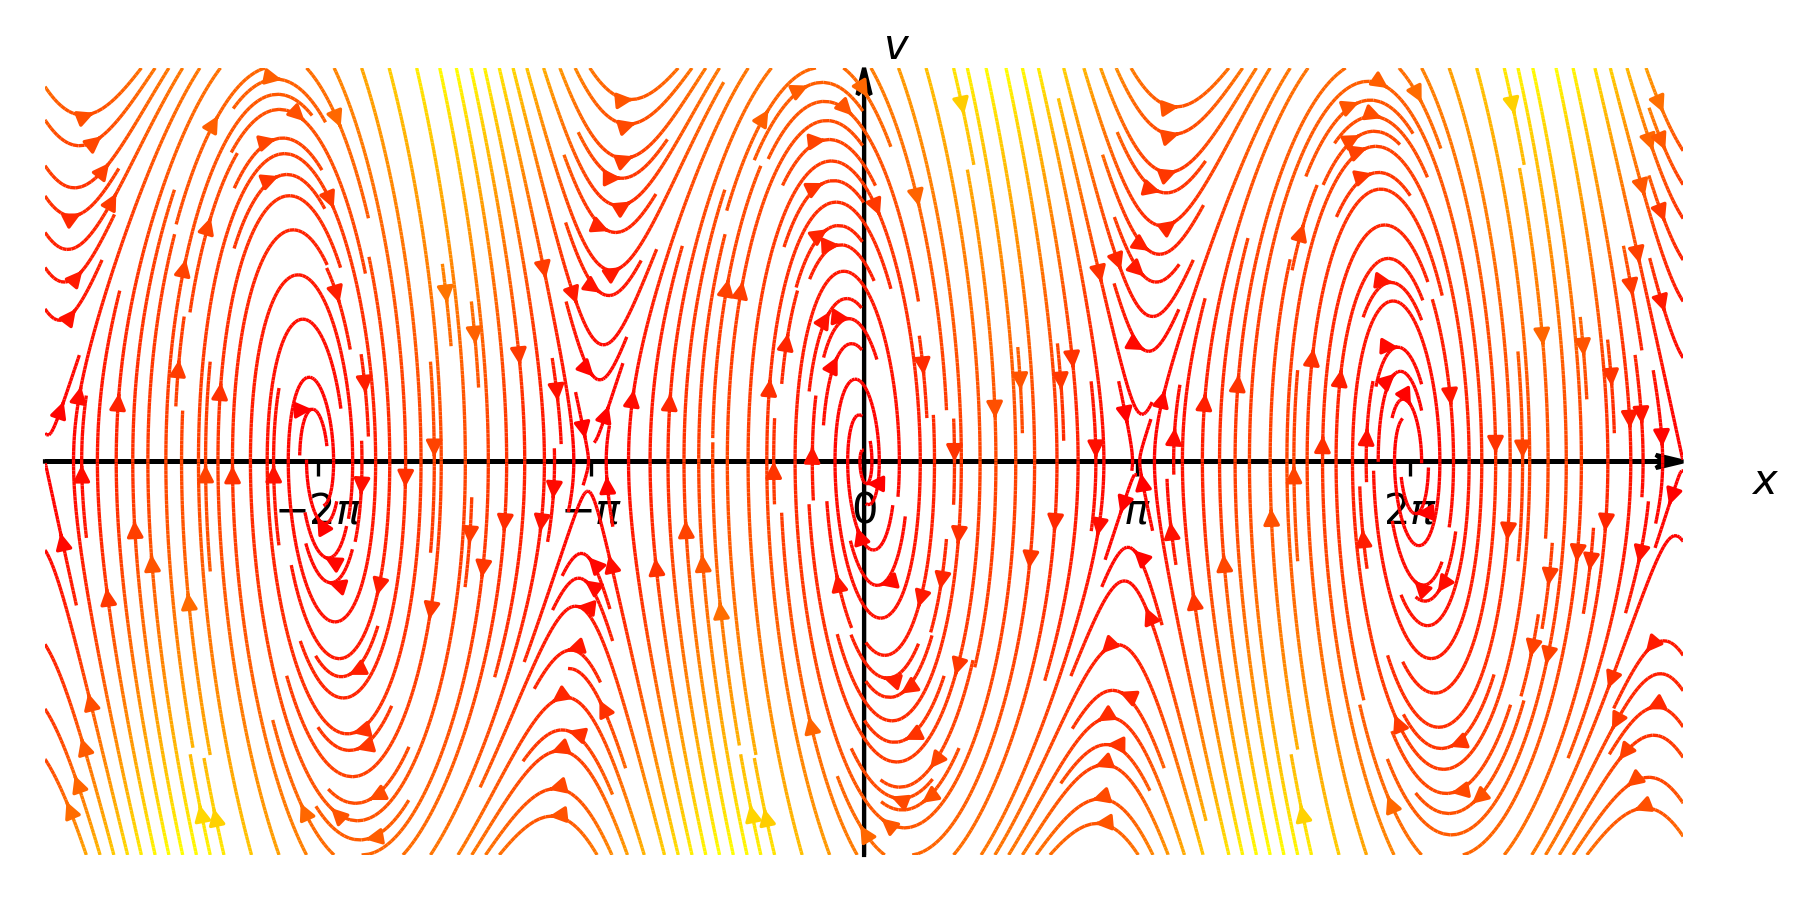
\includegraphics[width=0.5\textwidth]{figures/15_pendolo.png}
	\caption{\scriptsize Rappresentazione del pendolo smorzato nello spazio delle fasi, grossolanamente si riescono a distinguere le spirali ed i punti sella. I colori indicano la "velocità" nello spazio delle fasi ($\sqrt{\dot{x}^2+\dot{v}^2}$), il giallo indica zone con tale quantità minore, il rosso le zone in cui gli oggetti si muovono più "velocemente".}
        \label{fig:fig}
    \end{figure}
    Interessante notare come viene "rotta" la spirale all'aumentare del parametro $\gamma$:
    \begin{figure}[H]
        \centering
	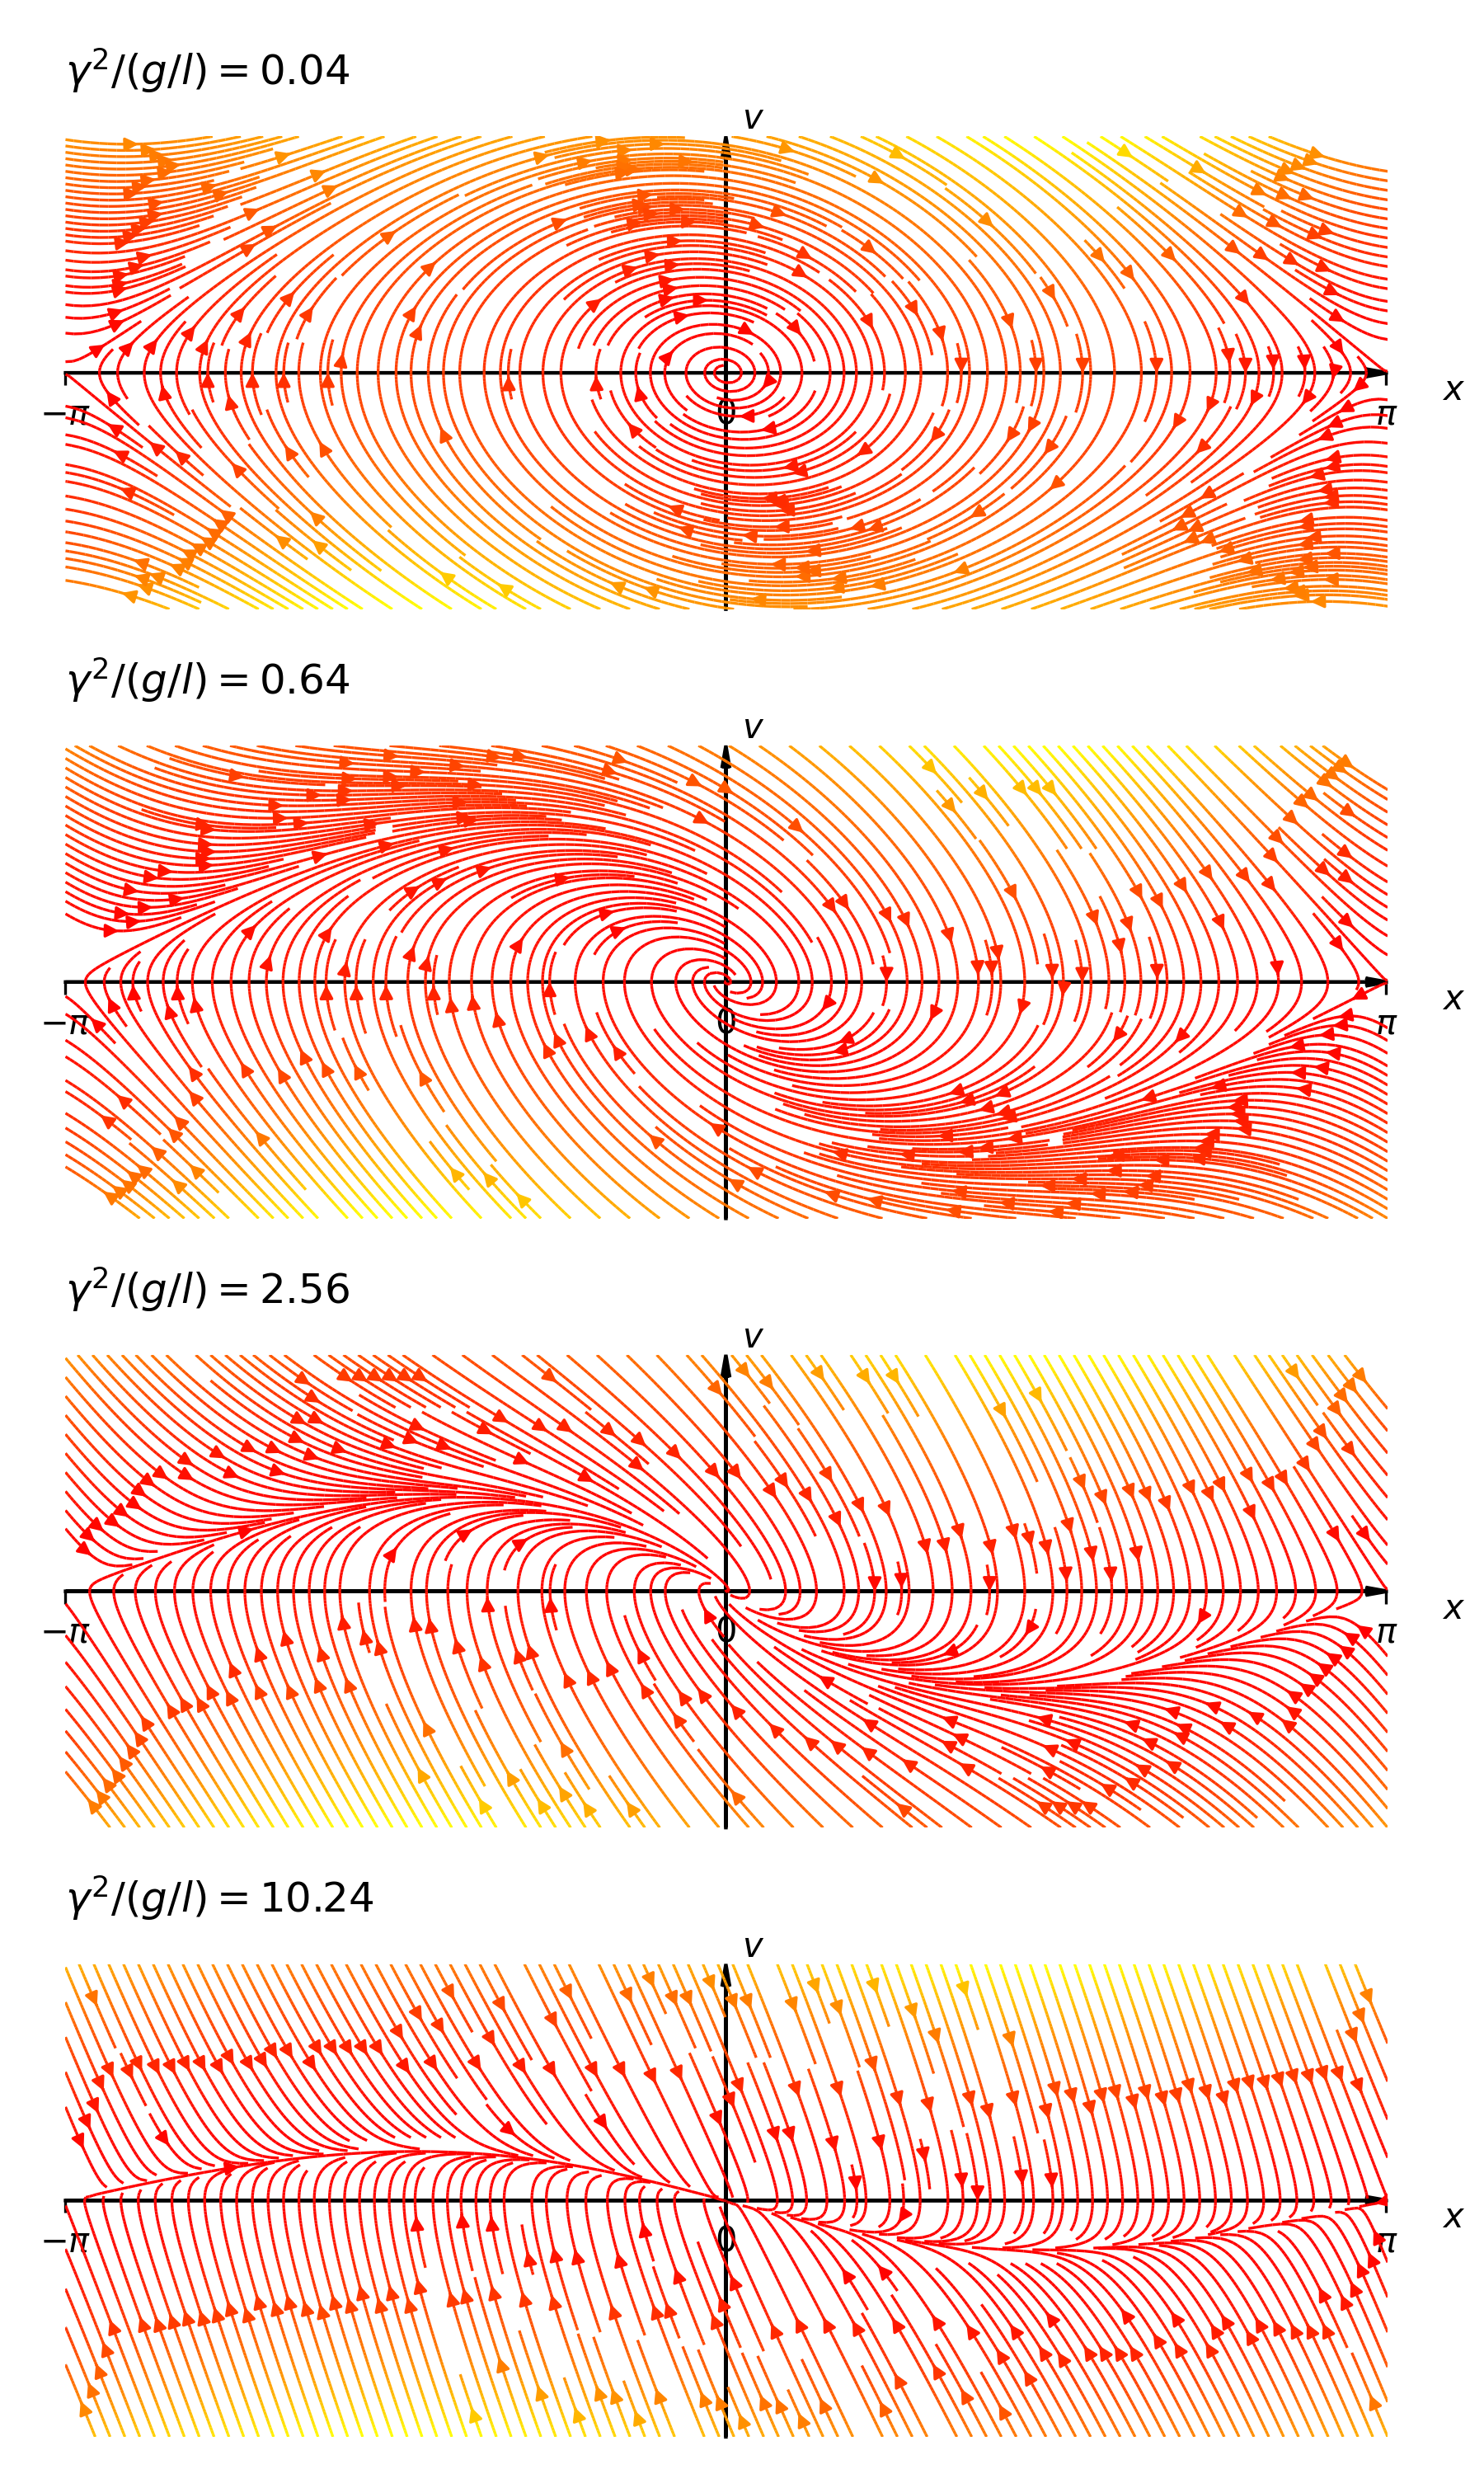
\includegraphics[width=0.5\textwidth]{figures/15_pendolo_accartoccio.png}
	\caption{\scriptsize Forma del flusso attorno all'origine al variare del rapporto $\gamma  / (g /l)$, si nota come la spirale sparisca all'aumentare di $\gamma$. Le linee di flusso tendono a collassare in modo anticipato su una curva oscillante.}
        \label{fig:figures-15_pendolo_accartoccio-png}
    \end{figure}
\end{exmp}
\noindent
\begin{exmp}[Equazioni di Lotka-Volterra]
    \[
        \begin{cases}
	    \dot{x} = x - xy\\
	    \dot{y} = - y + xy
        \end{cases}
    \] 
    In cui $x, y > 0$. \\
    I punti stazionari per queste equazioni sono (quando si annullano sia $\dot{x}$ che $\dot{y}$):
    \[\begin{aligned}
	& P_0 = (0,0) \\
	& P_1 = (1,1) 
    .\end{aligned}\]
    Le nurk lines invece sono le quattro rette:
    \[\begin{aligned}
        x = 0 \qquad x = 1\\
	y = 0 \qquad y = 1
    .\end{aligned}\]
    Passiamo direttamente al sistema linearizzato:
    \[
        \begin{pmatrix} \delta\dot{x} \\ \delta\dot{y} \end{pmatrix} =
	\begin{pmatrix} 
	  1-y & -x \\
          y & -1+x
        \end{pmatrix} 
	\begin{pmatrix} \delta x \\ \delta y \end{pmatrix} 
    .\] 
    Si tratta adesso di valutare i due punti fissi singolarmente per vedere di che tipo sono.\\
    Per l'origine degli assi si ha che la matrice $M$ è:
    \[
	M_{00} = 
        \begin{pmatrix} 
	1 & 0\\
        0 & -1
        \end{pmatrix} 
    .\] 
    La matrice è già in forma diagonale, quindi si ha un autovalore positivo ed uno negativo: l'origine è un punto iperbolico.\\
    Per quanto riguarda il punto $x=y=1$ si ha
    \[
	M_{11} = 
        \begin{pmatrix} 
	0 & -1\\
        1 & 0
        \end{pmatrix} 
    .\] 
    gli autovalori sono $\pm i$, quindi il punto è ellittico.
    \begin{figure}[H]
        \centering
	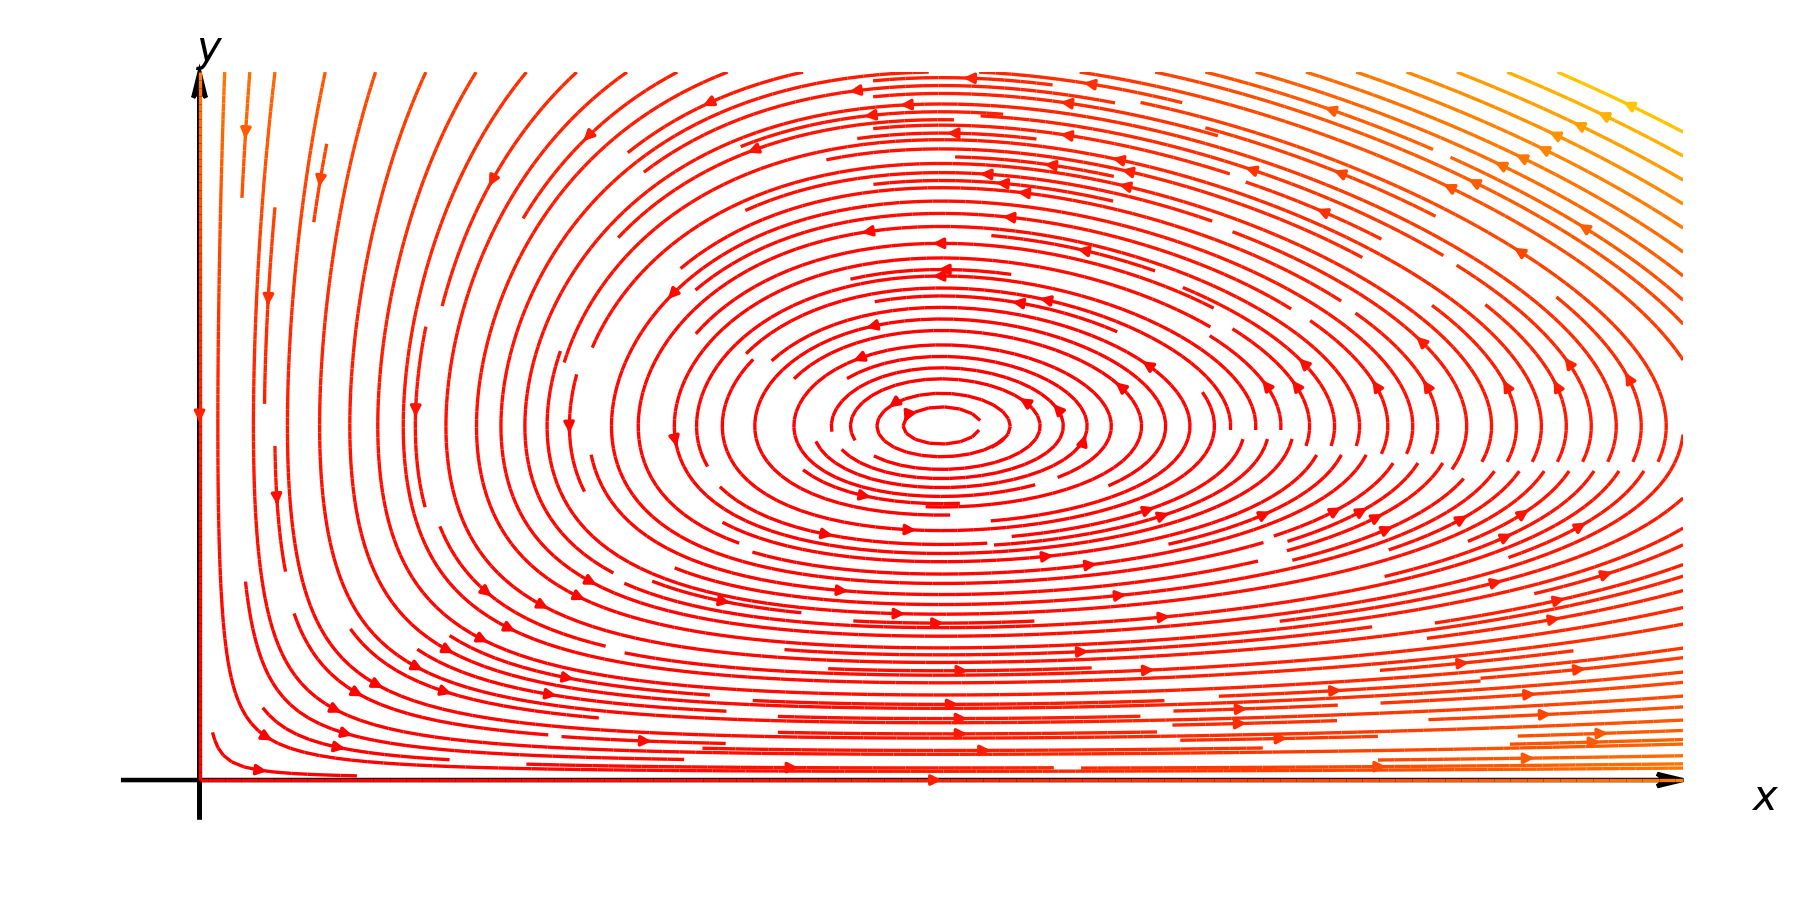
\includegraphics[width=0.5\textwidth]{figures/15_volterra.png}
        \caption{\scriptsize Flusso nello spazio delle fasi per il sistema di Lotka-Volterra.}
        \label{fig:figures-15_volterra-png}
    \end{figure}
    Questa equazione è studiata nel contesto della dinamica delle popolazioni, come già accennato nella primissima lezione.
\end{exmp}
\noindent
\begin{exmp}[Equazione non lineare incasinata]
    Prendiamo il sistema di equazioni:
    \[
        \begin{cases}
	    \dot{x} = x + y - x (x^2+y^2) \\
	    \dot{y}=- x + y - y(x^2+ y^2) 
        \end{cases}
    .\] 
    Non è chiaro dalle equazioni se vi è un punto fisso, una strategia vincente di soluzione è cambiare variabile.
    \[
        R^2=x^2+y^2
    .\] 
    Così facendo si ha che:
    \[
        \frac{\text{d} R^2}{\text{d} t} = R^2-R^4
    .\] 
    Quindi adesso cambiando nuovamente variabili si ottiene:
    \[
        \dot{z}=z-z^2
    .\] 
    Questa è l'unica equazione che dobbiamo studiare, stiamo infatti risolvendo il sistema in coordinate "radiali".\\
    I punti fissi in $z$ sono:
    \[\begin{aligned}
	& z = 0\\
	& z = 1
    .\end{aligned}\] 
    Valutare gli autovalori è più semplice in una dimensione:
    \[
	\delta\dot{z}=(1-2z) \delta z
    .\] 
    Quindi nel caso di $z=0$ abbiamo $\lambda =1$, quindi abbiamo un punto instabile. Nel caso di $z=1$ abbiamo $\lambda =-1$ e quindi un punto stabile.\\
    La grossa differenza dai sistemi visti in precedenza è che il punto $z=1$ è in realtà una varietà: $x^2+y^2=1$, di conseguenza non è semplicemente un punto stabile ma una intera varietà stabile.\\
    In altri termini tutti i punti del piano $x,y$ tenderanno a cadere sulla circonferenza di raggio unitario. 
\end{exmp}
\noindent
\clearpage
